\documentclass[a4paper]{article}
\usepackage{amsmath}
\usepackage{bm}
\usepackage{xcolor}
\usepackage{braket}
\usepackage{amssymb}
\usepackage{mathrsfs}
\usepackage{mathtools}
\usepackage{simplewick}
\begin{document}
	\title{chapter\;12}
	\date{ }
	\maketitle
\section{Application of scattering}
\subsection{decay process}
The differential transition probability for one pariticle decaying into some n-particle final state is conventionally called $d\Gamma$ $$d\Gamma=\frac{\text{diff. decay prob.}}{\text{unit time}}=\frac{1}{2E_{\bm{p}}}|A_{fi}|^2D$$
The life span thus $\Gamma$ is different between a rest and
a moving pariticle.Note that$$\frac{\text{rest decay prob.}}{\text{unit time}}=\Gamma=\frac{1}{2m}\sum_{\substack{\text{final}\\ \text{states}}}\int |A_{fi}|^2 D$$Thus$$\frac{\text{moving decay prob.}}{\text{unit time}}=\frac{m}{E_{\bm{p}}}\Gamma=\frac{d\tau}{dt}\Gamma<\Gamma$$Therefore,one can claim that a particle decays faster if it rests.
\par eg.Consider $\phi\rightarrow N+\bar{N}$ prcess.
\begin{figure}[htbp]
	\centering
	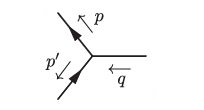
\includegraphics[width=0.6\textwidth,height=0.1\textheight]{18.png}
	\caption{$\phi\rightarrow N+\bar{N}$}
\end{figure}
To lowerest non zero order,$A_{fi}=-g$.Substitute into formular and yield$$\Gamma=\frac{g^2}{8\pi\mu E_T}|p_f|$$In center-of-momentum frame,$|\bm{p}_1|=|\bm{p}_2|=|\bm{p}_f|,E_T=2\sqrt{|\bm{p}_f^2+\mu^2|}=m$,thus$$\Gamma=\frac{g^2}{16\pi m^2}\sqrt{m^2-4\mu^2}$$One can see that the meson is not stable if $m>2\mu$.
\subsection{cross-section}
Consider a two particles initial state $\ket{i}=\sqrt{V}\ket{\bm{p}_1,\bm{p}_2}$,and these two moving with velocity $\bm{v}_1$ and $\bm{v}_2$ will encounter each other and scatter.It is easy to check that the particle density is 1 and thus$$\text{flux}=\frac{\text{particle density}\times V}{\text{area}\times\text{time}}=\frac{|\bm{v}_1-\bm{v}_2|At}{At}=|\bm{v}_1-\bm{v}_2|$$
\begin{figure}[htbp]
	\centering
	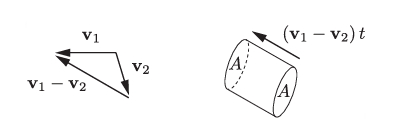
\includegraphics[width=0.6\textwidth]{17.png}
	\caption{flux for two particles}
\end{figure}
Then the differential cross-section is found to be$$d\sigma=\frac{\text{diff. trans. prob.}}{\text{unittime}\times\text{unit flux}}=\frac{1}{4E_1E_2}|A_{fi}|^2D\frac{1}{|\bm{v}_1-\bm{v}_2|}$$
Integral over all final state$$\sigma=\frac{1}{|\bm{v}_1-\bm{v}_2|}\frac{1}{4E_1E_2}\sum_{\substack{\text{final}\\ \text{states}}}\int|A_{fi}|^2D$$
Note that the factor $\frac{1}{4E_1E_2|\bm{v}_1-\bm{v}_2|}$ is not Lorentz invairiant,unless the transformation is confined in (0,1) plane,which does not change the geometrical shape of cross-section.
To proceed,in center-of-momentum frame,let
\begin{align*}
	&p_1=(E_1,p_i,0,0)\\
	&p_2=(E_2,-p_i,0,0)
\end{align*}
then
\begin{align*}
	E_1E_2|\bm{v}_1-\bm{v}_2|&=E_1E_2|\frac{p_i}{E_1}+\frac{p_i}{E_1}|\\&=(E_1+E_2)|p_i|=E_T|p_i|
\end{align*}
where $E_T$ is the total energy of two particles.
\par Finally,the cross-section in center-of-momentum can be expressed as$$\sigma=\frac{1}{4E_T|\bm{p}_i|}\sum_{\substack{\text{final}\\ \text{states}}}\int|A_{fi}|^2D$$
\subsection{optical theorem}
The optical theorem connects imaginary part of scarttering amplitude and cross-section$$Im\,A_{ii}=2E_T|p_{i}|\sigma$$
where $i$ indicates initial state.
\par Start from S-matrix $S^{\dagger}S=1$,then$$(S^{\dagger}-1)(S-1)=-(S-1)-(S^{\dagger}-1)$$Note that
\begin{align*}
	&\bra{f}S-1\ket{i}=iA_{fi}(2\pi)^4\delta^{(4)}(p_f-p_i)\\
	&\bra{f}(S-1)^{\dagger}\ket{i}=-iA_{if}^*(2\pi)^4\delta^{(4)}(p_f-p_i)\\
\end{align*}
Thus$$\bra{f}(S-1)^{\dagger}(S-1)\ket{i}=(2\pi)^4\delta^{(4)}(p_f-p_i)(iA^*_{if}-iA_{fi})$$
Another way to calculate left handside is use completeness relationship.
\begin{align*}
	&\bra{f}(S-1)^{\dagger}(S-1)\ket{i}=\sum_{m}\bra{f}(S-1)^{\dagger}\ket{m}\bra{m}(S-1)\ket{i}\\=&\sum_{r=1}^{\infty}\frac{1}{r!}\int\frac{d^3\bm{q}_1}{(2\pi)^32E_1}\cdots\frac{d^3\bm{q}_2}{(2\pi)^32E_2}\bra{f}(S-1)^{\dagger}\ket{q_1,\cdots q_r}\bra{q_1,\cdots q_r}(S-1)\ket{i}
\end{align*}
where there is correpondence $\ket{m}\leftrightarrow\ket{q_1,\cdots q_r}$ and vaccum is ignored as $(S-1)\ket{0}=0$.Simplify the expression by substuting
\begin{align*}
	&\bra{q_1\cdots q_r}(S-1)\ket{i}=iA_{mi}(2\pi)^4\delta^{(4)}(p_m-p_i)\\
	&\bra{f}(S-1)^{\dagger}\ket{q_1\cdots q_r}=-iA_{mf}^*(2\pi)^4\delta^{(4)}(p_f-p_m)
\end{align*}
then
\begin{align*}
	&\bra{f}(S-1)^{\dagger}(S-1)\ket{i}=\sum_{r=1}^{\infty}\frac{1}{r!}\prod_{n=1}^{r}\int \frac{d^3\bm{q}_n}{(2\pi)^32E_n}A^*_{mf}A_{mi}(2\pi)^8\delta^{(4)}(p_m-p_i)\delta^{(4)}(p_f-p_m)\\=&(2\pi)^4\delta^{(4)}(p_f-_i)\sum_{r=1}^{\infty}\frac{1}{r!}\prod_{n=1}^{r}\int\frac{d^3\bm{q}_n}{(2\pi)^32E_n}A^*_{mf}A_{mi}(2\pi)^4\delta^{(4)}(p_m-p_i)
\end{align*}
Now set $\ket{i}=\ket{f}$,and let $\ket{i}=\ket{\bm{p}_i,-\bm{p}_i}$(as was in the cross-section derivation part)
\begin{align*}
&2Im\,A_{ii}=\\
&i(A_{ii}^*-A_{ii})=\sum_{r=1}^{\infty}\frac{1}{r!}\prod_{n=1}^{r}\int\frac{d^3\bm{q}_n}{(2\pi)^32E_n}|A_{mi}|^2(2\pi)^4\delta^{(4)}(p_m-p_i)\\=&\sum_{\substack{\text{final}\\ \text{states}}}\int D|A_{fi}|^2=4E_T|\bm{p}_i|\sigma
\end{align*}
Therefore,$$Im\,A_{ii}=2E_T|\bm{p}_i|\sigma$$
\end{document}